\chapter{Registri e Organizzazione della Memoria}

\section{Introduzione}

I registri sono celle di memoria ultrarapide integrate nel processore. L'8086 dispone di 14 registri a 16 bit, suddivisi in 4 categorie: registri generali, registri puntatore, registri indice e registri segmento. La conoscenza approfondita dei registri è fondamentale per scrivere codice Assembly efficiente.

\section{Registri General Purpose}

L'8086 ha 4 registri general purpose a 16 bit, ciascuno divisibile in due registri a 8 bit.

\subsection{Registro AX (Accumulatore)}

\begin{definizione}
\textbf{AX} è il registro \emph{accumulatore}, utilizzato per operazioni aritmetiche, I/O e moltiplicazioni/divisioni.
\end{definizione}

\begin{itemize}
    \item \textbf{AX} (16 bit): Accumulatore completo
    \item \textbf{AH} (8 bit): Byte alto (High)
    \item \textbf{AL} (8 bit): Byte basso (Low)
\end{itemize}

\begin{center}
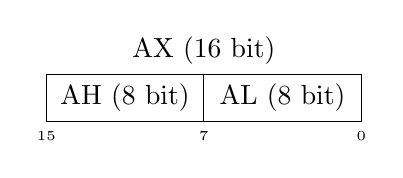
\begin{tikzpicture}
    \draw (0,0) rectangle (4,0.6);
    \draw (2,0) -- (2,0.6);
    \node at (1,0.3) {AH (8 bit)};
    \node at (3,0.3) {AL (8 bit)};
    \node[above] at (2,0.6) {AX (16 bit)};

    % Bit numbering
    \node[below, font=\tiny] at (0,0) {15};
    \node[below, font=\tiny] at (2,0) {7};
    \node[below, font=\tiny] at (4,0) {0};
\end{tikzpicture}
\end{center}

\textbf{Usi tipici}:
\begin{itemize}
    \item Operazioni aritmetiche generiche
    \item Istruzioni I/O (\texttt{IN AL, port} / \texttt{OUT port, AL})
    \item Moltiplicazione: risultato in AX (8 bit) o DX:AX (16 bit)
    \item Divisione: dividendo in AX (8 bit) o DX:AX (16 bit)
\end{itemize}

\subsection{Registro BX (Base)}

\begin{itemize}
    \item \textbf{BX}: Registro base per indirizzamento indiretto
    \item \textbf{BH} / \textbf{BL}: Byte alto/basso
\end{itemize}

\textbf{Usi tipici}:
\begin{itemize}
    \item Indirizzamento di array: \texttt{MOV AL, [BX]}
    \item Puntatore a strutture dati
    \item Calcoli generici
\end{itemize}

\subsection{Registro CX (Contatore)}

\begin{itemize}
    \item \textbf{CX}: Registro contatore per loop
    \item \textbf{CH} / \textbf{CL}: Byte alto/basso
\end{itemize}

\textbf{Usi tipici}:
\begin{itemize}
    \item Contatore in istruzioni \texttt{LOOP}, \texttt{LOOPE}, \texttt{LOOPNE}
    \item Contatore in operazioni su stringhe con prefisso \texttt{REP}
    \item Shift/rotate: CL specifica il numero di posizioni
\end{itemize}

\subsection{Registro DX (Dati)}

\begin{itemize}
    \item \textbf{DX}: Registro dati per I/O e operazioni estese
    \item \textbf{DH} / \textbf{DL}: Byte alto/basso
\end{itemize}

\textbf{Usi tipici}:
\begin{itemize}
    \item Indirizzamento porte I/O: \texttt{IN AL, DX} / \texttt{OUT DX, AL}
    \item Moltiplicazione 16 bit: risultato alto in DX, basso in AX
    \item Divisione 16 bit: dividendo in DX:AX
\end{itemize}

\subsection{Tabella riassuntiva}

\begin{table}[h]
\centering
\begin{tabular}{lllp{6cm}}
\toprule
\textbf{16 bit} & \textbf{8 bit H} & \textbf{8 bit L} & \textbf{Uso principale} \\
\midrule
AX & AH & AL & Accumulatore, I/O, moltiplicazioni \\
BX & BH & BL & Base per indirizzamento, puntatori \\
CX & CH & CL & Contatore loop, shift count \\
DX & DH & DL & Dati, porte I/O, divisioni \\
\bottomrule
\end{tabular}
\caption{Registri general purpose}
\end{table}

\section{Registri Puntatore e Indice}

Questi registri sono utilizzati per l'indirizzamento della memoria e non sono divisibili in byte.

\subsection{Stack Pointer (SP)}

\begin{definizione}
\textbf{SP} punta alla cima dello stack nel segmento SS. Lo stack cresce verso indirizzi decrescenti.
\end{definizione}

\begin{itemize}
    \item Utilizzato con \texttt{PUSH} e \texttt{POP}
    \item Automaticamente decrementato da \texttt{PUSH}, incrementato da \texttt{POP}
    \item Indirizzo stack: \texttt{SS:SP}
\end{itemize}

\subsection{Base Pointer (BP)}

\begin{itemize}
    \item \textbf{BP}: Puntatore base per accedere parametri e variabili locali
    \item Tipicamente usato con segmento SS: \texttt{[BP+offset]}
    \item Fondamentale nelle chiamate a procedure
\end{itemize}

\subsection{Source Index (SI)}

\begin{itemize}
    \item \textbf{SI}: Indice sorgente per operazioni su stringhe
    \item Usato con segmento DS: \texttt{DS:SI}
    \item Auto-incremento/decremento con istruzioni \texttt{LODS}, \texttt{MOVS}, \texttt{CMPS}
\end{itemize}

\subsection{Destination Index (DI)}

\begin{itemize}
    \item \textbf{DI}: Indice destinazione per operazioni su stringhe
    \item Usato con segmento ES: \texttt{ES:DI}
    \item Auto-incremento/decremento con istruzioni \texttt{STOS}, \texttt{MOVS}, \texttt{SCAS}
\end{itemize}

\subsection{Instruction Pointer (IP)}

\begin{definizione}
\textbf{IP} contiene l'offset della prossima istruzione da eseguire nel segmento CS. Non è direttamente modificabile, ma cambia con istruzioni di salto e chiamate.
\end{definizione}

\begin{itemize}
    \item Indirizzo istruzione corrente: \texttt{CS:IP}
    \item Modificato da: \texttt{JMP}, \texttt{CALL}, \texttt{RET}, \texttt{INT}, \texttt{IRET}
    \item Automaticamente incrementato dopo ogni istruzione
\end{itemize}

\section{Registri Segmento}

I 4 registri segmento definiscono le basi dei segmenti di memoria.

\subsection{Code Segment (CS)}

\begin{itemize}
    \item \textbf{CS}: Segmento codice, contiene le istruzioni del programma
    \item Indirizzo istruzione: \texttt{CS:IP}
    \item Modificabile solo con \texttt{JMP FAR}, \texttt{CALL FAR}, \texttt{RET FAR}
\end{itemize}

\subsection{Data Segment (DS)}

\begin{itemize}
    \item \textbf{DS}: Segmento dati, contiene variabili globali
    \item Usato implicitamente da: \texttt{[BX]}, \texttt{[SI]}, \texttt{[DI]}
    \item Modificabile con \texttt{MOV DS, AX}
\end{itemize}

\subsection{Stack Segment (SS)}

\begin{itemize}
    \item \textbf{SS}: Segmento stack, area per \texttt{PUSH}/\texttt{POP}
    \item Indirizzo cima stack: \texttt{SS:SP}
    \item Usato implicitamente da \texttt{[BP]}
\end{itemize}

\subsection{Extra Segment (ES)}

\begin{itemize}
    \item \textbf{ES}: Segmento extra per operazioni su stringhe
    \item Usato implicitamente da \texttt{DI} in \texttt{STOS}, \texttt{MOVS}, \texttt{SCAS}
    \item Utile per copiare dati tra segmenti
\end{itemize}

\begin{attenzione}
I registri segmento \textbf{non possono essere modificati direttamente}. Bisogna passare attraverso un registro general purpose:

\begin{lstlisting}
; CORRETTO
MOV AX, 1000h
MOV DS, AX

; ERRORE - non consentito
MOV DS, 1000h
\end{lstlisting}
\end{attenzione}

\section{Organizzazione della Memoria}

\subsection{Modello di memoria segmentata}

Lo spazio di indirizzamento dell'8086 (1 MB) è organizzato in segmenti sovrapposti:

\begin{center}
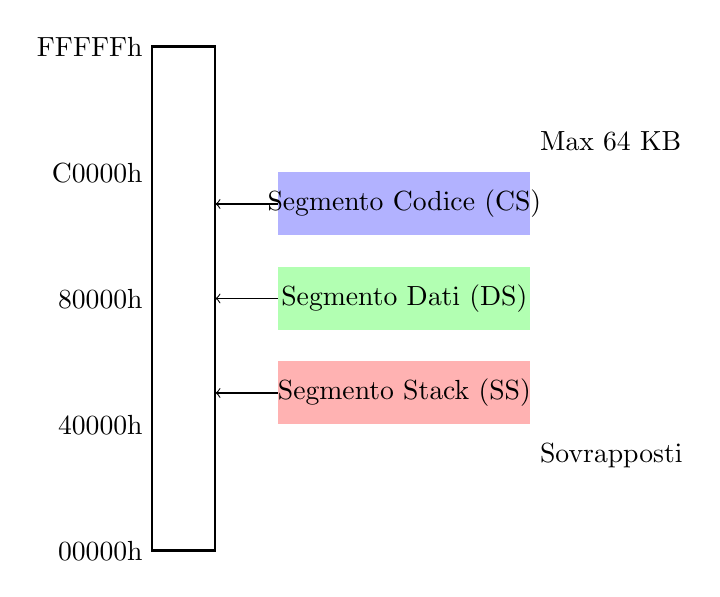
\begin{tikzpicture}[scale=0.8]
    % Memoria lineare
    \draw[thick] (0,0) rectangle (1,8);
    \node[left] at (0,8) {FFFFFh};
    \node[left] at (0,6) {C0000h};
    \node[left] at (0,4) {80000h};
    \node[left] at (0,2) {40000h};
    \node[left] at (0,0) {00000h};

    % Segmento codice
    \fill[blue!30] (2,5) rectangle (6,6);
    \node at (4,5.5) {Segmento Codice (CS)};

    % Segmento dati
    \fill[green!30] (2,3.5) rectangle (6,4.5);
    \node at (4,4) {Segmento Dati (DS)};

    % Segmento stack
    \fill[red!30] (2,2) rectangle (6,3);
    \node at (4,2.5) {Segmento Stack (SS)};

    % Frecce
    \draw[<-] (1,5.5) -- (2,5.5);
    \draw[<-] (1,4) -- (2,4);
    \draw[<-] (1,2.5) -- (2,2.5);

    \node[right] at (6,6.5) {Max 64 KB};
    \node[right] at (6,1.5) {Sovrapposti};
\end{tikzpicture}
\end{center}

\subsection{Layout tipico di un programma .COM}

\begin{center}
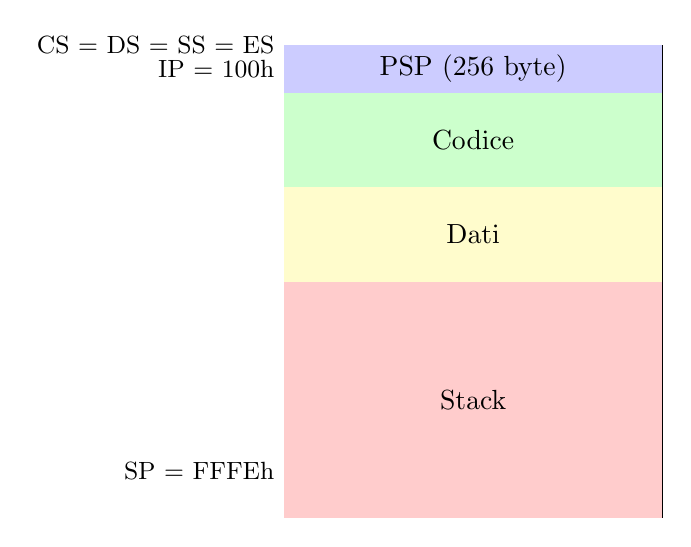
\begin{tikzpicture}[scale=1.2]
    \draw (0,0) rectangle (4,5);

    \fill[blue!20] (0,4.5) rectangle (4,5);
    \node at (2,4.75) {PSP (256 byte)};

    \fill[green!20] (0,3.5) rectangle (4,4.5);
    \node at (2,4) {Codice};

    \fill[yellow!20] (0,2.5) rectangle (4,3.5);
    \node at (2,3) {Dati};

    \fill[red!20] (0,0) rectangle (4,2.5);
    \node at (2,1.25) {Stack};

    \node[left, font=\small] at (0,5) {CS = DS = SS = ES};
    \node[left, font=\small] at (0,4.75) {IP = 100h};
    \node[left, font=\small] at (0,0.5) {SP = FFFEh};
\end{tikzpicture}
\end{center}

\begin{nota}
Nei programmi \textbf{.COM}, tutti i registri segmento puntano allo stesso indirizzo. L'intera immagine del programma (codice, dati, stack) risiede in un unico segmento di 64 KB. Il Program Segment Prefix (PSP) occupa i primi 256 byte.
\end{nota}

\subsection{Layout programma .EXE}

Nei file .EXE i segmenti sono separati:

\begin{itemize}
    \item \textbf{CS}: Segmento codice (istruzioni)
    \item \textbf{DS}: Segmento dati (variabili globali)
    \item \textbf{SS}: Segmento stack (separato da codice e dati)
    \item \textbf{ES}: Tipicamente uguale a DS all'avvio
\end{itemize}

\section{Convenzioni di utilizzo}

\begin{table}[h]
\centering
\small
\begin{tabular}{lp{9cm}}
\toprule
\textbf{Operazione} & \textbf{Registri tipici} \\
\midrule
Moltiplicazione 8 bit & AL × operando $\rightarrow$ AX \\
Moltiplicazione 16 bit & AX × operando $\rightarrow$ DX:AX \\
Divisione 8 bit & AX ÷ operando $\rightarrow$ AL (quoziente), AH (resto) \\
Divisione 16 bit & DX:AX ÷ operando $\rightarrow$ AX (quoziente), DX (resto) \\
Loop counter & CX (decrementato automaticamente) \\
String source & DS:SI \\
String destination & ES:DI \\
Procedure stack frame & SS:BP \\
I/O a 8 bit fisso & AL + numero porta immediato \\
I/O variabile & AL/AX + DX (numero porta) \\
\bottomrule
\end{tabular}
\caption{Convenzioni d'uso dei registri}
\end{table}

\section{Esempi pratici}

\begin{esempio}
Sommare due numeri a 16 bit:

\begin{lstlisting}
; Somma: 1234h + 5678h = 68ACh
MOV AX, 1234h     ; AX = 1234h
MOV BX, 5678h     ; BX = 5678h
ADD AX, BX        ; AX = 68ACh, BX immutato
\end{lstlisting}
\end{esempio}

\begin{esempio}
Accesso a byte alto e basso:

\begin{lstlisting}
MOV AX, 1234h     ; AX = 1234h
MOV BL, AL        ; BL = 34h (byte basso)
MOV BH, AH        ; BH = 12h (byte alto)
; Ora BX = 1234h
\end{lstlisting}
\end{esempio}

\begin{esempio}
Indirizzamento indiretto con BX:

\begin{lstlisting}
.DATA
array DB 10h, 20h, 30h, 40h

.CODE
MOV BX, OFFSET array   ; BX punta all'array
MOV AL, [BX]           ; AL = 10h (primo elemento)
INC BX                 ; BX punta al secondo elemento
MOV AL, [BX]           ; AL = 20h
\end{lstlisting}
\end{esempio}

\section{Riepilogo}

\begin{itemize}
    \item L'8086 ha 14 registri a 16 bit
    \item I 4 registri general purpose (AX, BX, CX, DX) sono divisibili in byte
    \item SP punta allo stack, BP ai parametri, SI/DI alle stringhe
    \item I 4 registri segmento (CS, DS, SS, ES) definiscono le basi dei segmenti
    \item IP contiene l'offset della prossima istruzione
    \item I programmi .COM usano un unico segmento, i .EXE hanno segmenti separati
\end{itemize}

\section{Esercizi}

\begin{esercizio}[2.1]
Dato \texttt{AX = 1234h}, scrivere le istruzioni per:
\begin{enumerate}[label=\alph*)]
    \item Azzerare solo AL mantenendo AH invariato
    \item Azzerare solo AH mantenendo AL invariato
    \item Scambiare AH e AL
\end{enumerate}
\end{esercizio}

\begin{esercizio}[2.2]
Spiegare la differenza tra \texttt{MOV AX, BX} e \texttt{MOV AX, [BX]}.
\end{esercizio}

\begin{esercizio}[2.3]
Perché non è possibile eseguire \texttt{MOV DS, 1000h}? Come si risolve?
\end{esercizio}

\begin{esercizio}[2.4]
Calcolare l'indirizzo fisico di \texttt{SS:SP = 2000h:FFFEh}. Se si esegue \texttt{PUSH AX}, qual è il nuovo valore di SP e l'indirizzo fisico corrispondente?
\end{esercizio}

\begin{esercizio}[2.5]
In un programma .COM, se tutti i segmenti valgono 1000h e IP = 0100h, qual è l'indirizzo fisico della prima istruzione?
\end{esercizio}
